% The Clever Algorithms Project: http://www.CleverAlgorithms.com
% (c) Copyright 2011 Jason Brownlee. Some Rights Reserved. 
% This work is licensed under a Creative Commons Attribution-Noncommercial-Share Alike 2.5 Australia License.

% Name
% The algorithm name defines the canonical name used to refer to the technique, in addition to common aliases, abbreviations, and acronyms. The name is used in terms of the heading and sub-headings of an algorithm description.
\section{BFGS Method} 
\label{sec:bfgs}
\index{Broyden-Fletcher-Goldfarb-Shanno Method}
\index{BFGS Method}
\index{Variable Metric Method}
\index{L-BFGS}
\index{Limited Memory BFGS}
\index{BFGS-B}

% other names
% What is the canonical name and common aliases for a technique?
% What are the common abbreviations and acronyms for a technique?
\emph{BFGS Method, BFGS, Broyden-Fletcher-Goldfarb-Shanno Method.}

% Taxonomy: Lineage and locality
\subsection{Taxonomy}
% To what fields of study does a technique belong?
BFGS is an optimization method for multidimensional nonlinear unconstrained functions.
% What are the closely related approaches to a technique?
BFGS belongs to the family of quasi-Newton (Variable Metric) optimization methods that make use of both first-derivative (gradient) and second-derivative (Hessian matrix) based information of the function being optimized. More specifically, it is a quasi-Newton method which means that it approximates the second-order derivative rather than compute it directly. It is related to other quasi-Newton methods such as the DFP Method, Broyden's method and the SR1 Method. 
% extensions
Two popular extension of BFGS is L-BFGS (Limited Memory BFGS) which has lower memory resource requirements and L-BFGS-B (Limited Memory Boxed BFGS) which extends L-BFGS and imposes box constraints on the method. 

% Strategy: Problem solving plan
% The strategy is an abstract description of the computational model. The strategy describes the information processing actions a technique shall take in order to achieve an objective. The strategy provides a logical separation between a computational realization (procedure) and a analogous system (metaphor). A given problem solving strategy may be realized as one of a number specific algorithms or problem solving systems. The strategy description is textual using information processing and algorithmic terminology.
\subsection{Strategy}
% What is the information processing objective of a technique?
The information processing objective of the BFGS Method is to locate the extremum of a function. 
% What is a techniques plan of action?
This is achieved by iteratively building up a good approximation of the inverse Hessian matrix.
Given an initial starting position, it prepares an approximation of the Hessian matrix (square matrix of second-order partial derivatives). It then repeats the process of computing the search direction using the approximated Hessian, computes an optimum step size using a Line Search then, updates the position, and updates the approximation of the Hessian. The method for updating the Hessian each iteration is called the BFGS rule which insures the updated matrix is positive definite.

% Heuristics: Usage guidelines
% The heuristics element describe the commonsense, best practice, and demonstrated rules for applying and configuring a parameterized algorithm. The heuristics relate to the technical details of the techniques procedure and data structures for general classes of application (neither specific implementations not specific problem instances). The heuristics are described textually, such as a series of guidelines in a bullet-point structure.
\subsection{Heuristics}
% What are the suggested configurations for a technique?
% What are the guidelines for the application of a technique to a problem instance?

\begin{itemize}
	\item It requires a function where the the functions gradient (first partial derivative) can be computed at arbitrary points.
	\item It does not require second-order derivatives as it approximates the Hessian matrix, making it less computationally expensive compared to Newton's method.
	\item It requires a relatively large memory footprint, as it maintains an $n*n$ Hessian matrix, where $n$ is the number of variables. This is a limitation on the methods scalability.
	\item The rate of convergence is superlinear and the computational cost of each iteration is $O(n^2)$ \cite{Nocedal1999}.
	\item The L-BFGS extension to BFGS is intended for functions with very large numbers of parameters ($>1000$).
	\item The stopping condition is typically a minimum change is response or a minimum gradient.
	\item BFGS is somewhat robust and self correcting in terms of the search direction and as such it does not require the use of exact line searches when determining the step size.
\end{itemize}

% sample script in R
\subsection{Code Listing}
% listing
Listing~\ref{stats_bfgs} provides a code listing of the BFGS method in R solving a two-dimensional nonlinear optimization function. Figure~\ref{plot:bfgs_result} provides a plot of the test problem with the located minimum highlighted.

% algorithm and package
The example uses the \texttt{optim()} function in the \texttt{stats} core package configured to use the BFGS method \cite{RDevelopmentCoreTeam2011a}. The \texttt{optim()} function is for General-purpose Optimization, for more information on this library type: \texttt{library(help="stats")}, and for more information on the function type: \texttt{?optim}.

% problem
The test problem is the Rosenbrock function in two-dimensions where the optimum is at $x,y=1$. The starting position for the algorithm is taken as a random point $x,y \in [-3,3]$. The gradient for this function is specified and is used by the optimization method.

% TODO consider capturing algorithm progression (using par)

\lstinputlisting[firstline=7,language=r,caption={Example of BFGS in R using the \texttt{optim()} function in the \texttt{stats} core package.}, label=stats_bfgs]{../src/algorithms/optimization/stats_bfgs.R}

\begin{figure}[htp]
\centering
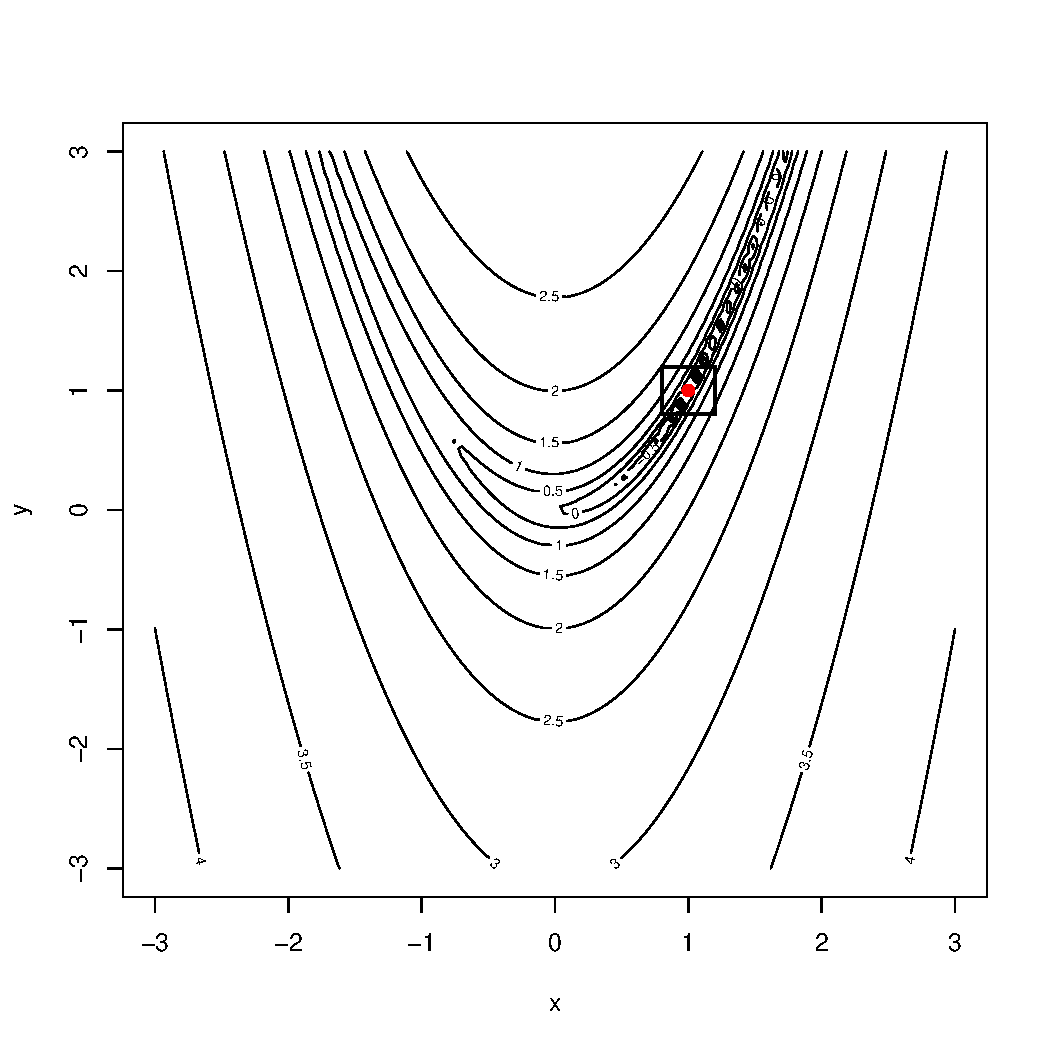
\includegraphics[scale=0.45]{a_optimization/bfgs_result.pdf}
\caption{Contour plot of the Rosenbrock function with the located minimum highlighted.}
\label{plot:bfgs_result}
\end{figure}

% other packages
The \texttt{optim()} function in the \texttt{stats} core package also offers an implementation of BFGS with both the Limited Memory (L-BFGS) and box constraint (BFGS-B) extensions based on the FORTRAN implementation described by Zhu et~al.\ \cite{Zhu1997}. The \texttt{gsl} package in the \texttt{multimin()} function provides an implementation of BFGS method that makes use of the GNU Scientific Library \cite{Hankin2011}.

% References: Deeper understanding
% The references element description includes a listing of both primary sources of information about the technique as well as useful introductory sources for novices to gain a deeper understanding of the theory and application of the technique. The description consists of hand-selected reference material including books, peer reviewed conference papers, journal articles, and potentially websites. A bullet-pointed structure is suggested.
\subsection{References}
% What are the primary sources for a technique?
% What are the suggested reference sources for learning more about a technique?

% primary sources
\subsubsection{Primary Sources}
% seminal 
The BFGS method was published by four authors at the same time in 1970: Broyden \cite{Broyden1970}, Fletcher \cite{Fletcher1970}, Goldfarb \cite{Goldfarb1970}, and Shanno \cite{Shanno1970}.
% extensions
The L-BFGS method was described by Nocedal \cite{Nocedal1980} and the L-BFGS-B extension was described by Byrd et~al.\ \cite{Byrd1995}.

% more info
\subsubsection{More Information}
% books
Nocedal and Wright provide a full description of the BFGS, L-BFGS and L-BFGS-B methods as well as full range of Quasi-Newton methods in their text on numerical optimization \cite{Nocedal1999}.
Press et~al.\ provide a good summary of the method with sample code in the C programming language \cite{Press2007} (Chapter 10.9).



% END
